\chapter{Non-linearities identification}

\section{Non-linear gain}
As previously mentioned the motor has shown its non-linear behaviour in some occasions, especially for the control of 2-DOF. \\
During the initial identification stage it was observed that the gain of the motor, i.e.: $\frac{1}{R}$ was input-varying, therefore non-linear. This was not seem as a problem, since it is a type of non-linearity whose sector is $[\alpha, \beta]$ with $\alpha > 0, \beta <M < \infty, M \in \mathbb{R}$. Therefore with a high-gain feedback loop, simply with an integrator, it's possible to linearise this effect. \\ \\
Obviously, since the poles of the motor is not changing  it means that either $\frac{R}{L}$ is a constant, with $R,L$ varying at the same velocity, which seems improbable, or that there is a non-linear gain that can be modelled as:
\begin{equation}
i(t)=\frac{1}{Ls+R} f(v)v = \frac{1}{Ls+R} g(v)
\end{equation}
Where $M(s)$ is the standard linear form of the motor, as previously presented, and $g: \mathbb{R} \to \mathbb{R}, \frac{dg}{dv} \in [\alpha, \beta]$.
Moreover, it seems to be a function with different behaviour for $v>0, v<0$. \\ \\Because of this, an identification process for both $v$ negative and positive was conducted.

Let the ideal current given by the following expression, where $R=1.3 \Omega, L=0.0024 H$.
\begin{equation}
i_{id}=\frac{1}{Ls+R} v(t)
\end{equation}
Then the real current is:
\begin{equation}
i(t)=  i_{id} f(v)
\end{equation}
Next we modelled $f(v)$ as a cubic function:
\begin{equation}
f(v) = \alpha+\beta v + \gamma v^2+\delta v^3
\end{equation}
And used a least squares procedure to identify $(\alpha, \beta, \gamma)$.
As a reference signal a step generator signal $r(t)$ was used with increasing voltage and period $5$ seconds, with $r(t) \in [-5,5]$. Next we used the procedure aforementioned only on the steady state portion  of the  measured current $i(t)$.\\ \\
Finally we can model $f(v)$ in the following way:
\begin{equation}
f(v(t)) = \begin{cases}
0.6564+0.1712v-0.0317v^2+0.0044v^3 \quad v>0 \\
-0.21-1.1397v-0.2756v^2-0.0226v^3 \quad v< 0
\end{cases}
\end{equation}
And $g(v) =f(v)v$.
  \begin{figure}[!h]
  \centering
  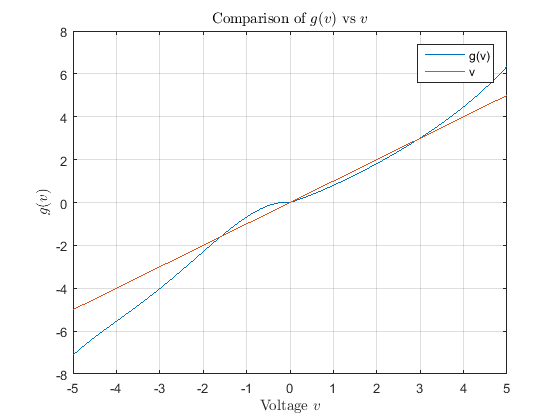
\includegraphics[width=0.5\textwidth]{img/nonlinear_gain.png}
  \caption{Plot of $g(v),v$.}
\end{figure}
\section{Static friction}
\section{Motor cogging identification}
It was found that for low voltage the motor acts as if the voltage is $0$, therefore the current and consequently the torque is $0$.\\
This is  a type of static friction, though it's not a mechanical one. In fact, if it was a mechanical one we would see the current increase but the shaft of the motor don't rotate until the torque is big enough to counteract the static friction effect. In this case is more an electrical type of static friction, called \emph{cogging} effect. \\ \\
COPIATO DA WIKI \\
Cogging torque of electrical motors is the torque due to the interaction between the permanent magnets of the rotor and the stator slots of a Permanent Magnet (PM) machine. This torque is position dependent and its periodicity per revolution depends on the number of magnetic poles and the number of teeth on the stator.Cogging torque results in torque as well as speed ripple; however, at high speed the motor moment of inertia filters out the effect of cogging torque.
\\ \\
In figure \ref{fig:curposvolt} such effect is shown. On the left plot it's visible that when the input voltage $v(t)$ for $|v(t)|< c$, the output current is $0$. Since the torque is proportional to the current, also the torque is $0$. On the right plot is visible the effect on the cart: when the cart starts to move, after having overcome the static friction, it stops because the torque goes to $0$ because the current is $0$. But this effect does not happen because of mechanical static friction, otherwise we would not see a flat current curve.  \\ \\
How can we model such effect? It's some kind of dead-zone effect, and we can model it such that the real voltage entering the motor is:
\begin{equation}
v_{real}(t) = \begin{cases}
0 \quad |v(t)| < c \\
v(t) \quad |v(t)| \geq c
\end{cases}
\end{equation}
Where $c \in \mathbb{R}$ needs to be identified. For this purpose, notice that inside the dead-zone the current is a white noise signal. Therefore we should find a constant $\alpha$ such that the signal $|i(t)| < \alpha$ is a white noise signal. We can make use of the fact that $v(t) \in C^{\infty}$ signal, find a set $\hat{t} = \{ t \in \mathbb{R}: |v(t)| < c \}$ and check the whiteness of the current in that set $\hat{t}$. Since $v$ is continuous, that set is measurable (using the Lebesgue measure). Also the current is continuous, therefore it's also continuous on that set. For this purpose the following identification procedure was used:
\begin{enumerate}
\item Use as voltage input a sinusoid with frequency pulsation $\omega = 1.25$ \SI{}{\radian \per \second}. 
\item Choose $c \in [0, \text{max}(v(t))]$, where $v(t)$ is the input voltage. Consider only the voltage that satisfies $|v(t)| < c$.
\item Run the Anderson Whiteness Test on the current for those values of $t$ where $|v(t)|<c$, with margin of tolerance of $1$\%.
\item {If the signal is not white, run again the test with $\alpha_{new}=\alpha-\Delta$,  where $0<\Delta < \alpha$. In our case $\Delta$ is fixed with value $10^{-2}$. In case the signal is white, stop. Notice that the bisection method cannot be used.}
\end{enumerate}
  \begin{figure}[!tbh]
  \centering
  \subfloat[Current vs Voltage plot]{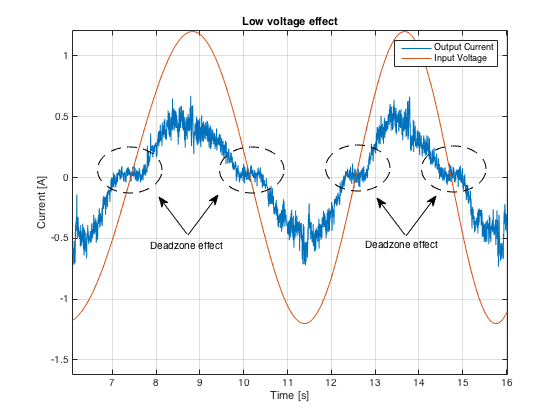
\includegraphics[width=0.5\textwidth]{img/deadzone1.png}}
  \hfill
  \subfloat[Current vs Position plot]{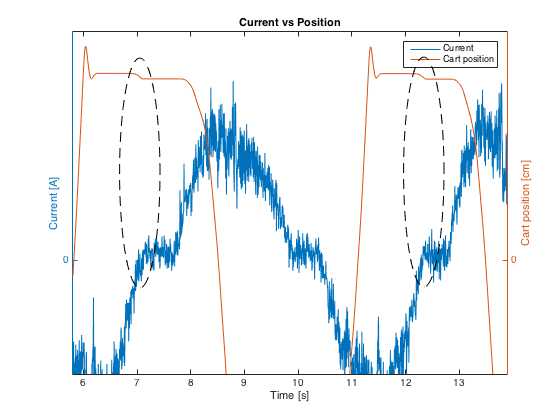
\includegraphics[width=0.5\textwidth]{img/deadzone2.png}}
  \caption{On the left: plot of the input voltage and output current. The deadzone effect on the current sets the current to 0 for small $v$. On the right  we can see the effect on the position of the cart.}
    \label{fig:curposvolt}
\end{figure}
Running this test gives an approximate value of $c \approx 0.35$ \SI{}{\volt}. The simulated current, using the parameters identified for the motor, is shown in figure \ref{fig:deadzone_sim}. Moreover, using the cost function  mentioned at the beginning of this part, we obtain a fit value of $0.89$ on the validation data (done using a different sinusoid). \\ \\
Instead if we minimise a least squares problem $J = \frac{1}{2} \sum_{t=0}^T (i_{sim}(t) -i_{real}(t))^2$, using the \emph{Genetic Algorithm} implemented in Matlab, gives a value of $c =0.4621$.
  \begin{figure}[!h]
  \centering
  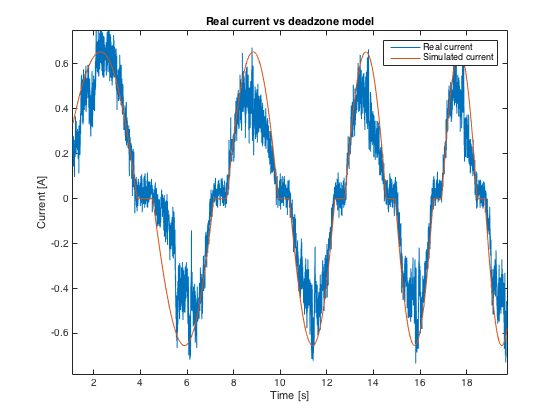
\includegraphics[width=0.5\textwidth]{img/deadzone3.png}
  \caption{Identified model vs real current.}
    \label{fig:deadzone_sim}
\end{figure}
\section{Motor mechanical static friction}

